\documentclass[../CIT217_RHEL124_LabJournal.tex]{subfiles}

\begin{document}

%%%%%%%%%%%%%%%%%%%%%%%%%%%%%%%%%%%%%%%%%%%%%%%%%%%%%
%%%%%%%%%%%%%%%%%%%%%%%%%%%%%%%%%%%%%%%%%%%%%%%%%%%%%

\chapter[RHEL 124 Labs 1 \& 2]{RHEL Labs\linebreak[1] 1 \& 2 \hspace*{\fill}{\date}}
\noindent\textbf{{RHEL 124 Labs 1 \& 2} \hspace*{\fill}{\textbf{CIT 217}}}\linebreak[1]
{{Spring 2020} \hspace*{\fill}{Chaz Davis}}                             
%===================================
%===================================
\mysection{\textbf{Part 1: Chapter 1 Questions}}

\mysubsection{1}{Provide the output of a sucessful password change from the CLI}

\begin{center}
	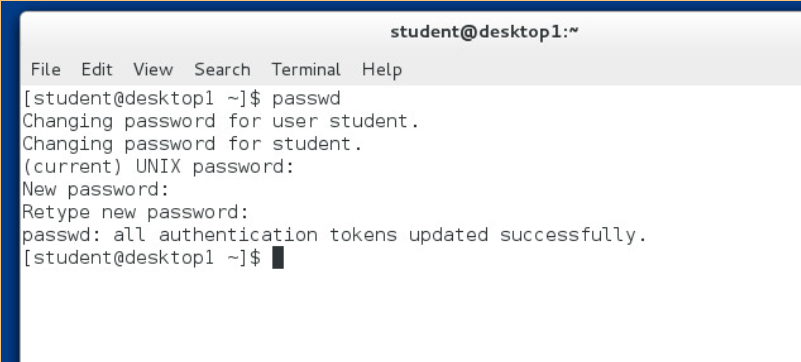
\includegraphics[scale=0.3]{Figures/2020-02-01-172540_801x362_scrot.png}
\end{center}

\mysubsection{2}{From the CLI, enter the command whoami and provide the output}
\begin{center}
	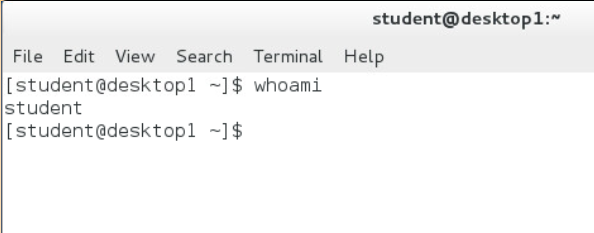
\includegraphics[scale=0.4]{Figures/2020-02-01-173144_594x233_scrot.png}
\end{center}

\mysubsection{3}{From the CLI, enter the command date +\%D-\%r and provide the
output}

\begin{center}
	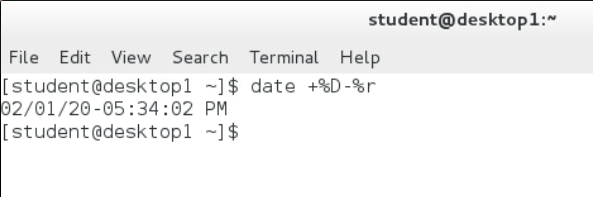
\includegraphics[scale=0.4]{Figures/2020-02-01-173412_593x197_scrot.png}
\end{center}

\mysubsection{4}{Using File, determine what type of file is /etc./networks}

\begin{center}
	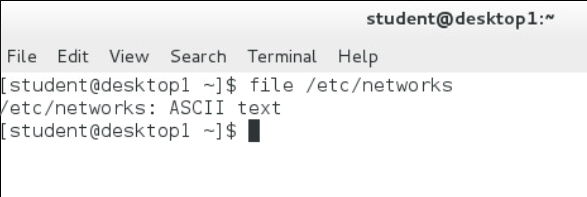
\includegraphics[scale=0.4]{Figures/2020-02-01-173553_587x197_scrot.png}
\end{center}

\newpage
\mysubsection{5}{Provide the top 5 lines of the file /etc/resolv.conf}

\begin{center}
	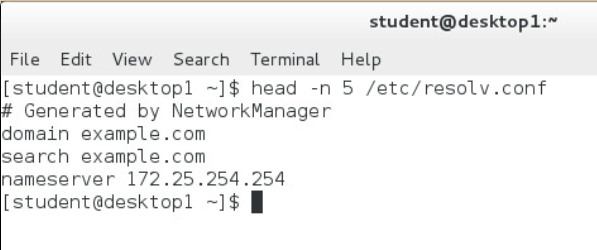
\includegraphics[scale=0.4]{Figures/2020-02-01-173753_597x250_scrot.png}
\end{center}

\mysubsection{6}{List your CLI history. Provide the output}

\begin{figure}[!hbt]
\begin{minipage}[c]{0.4\linewidth}
  \centering
	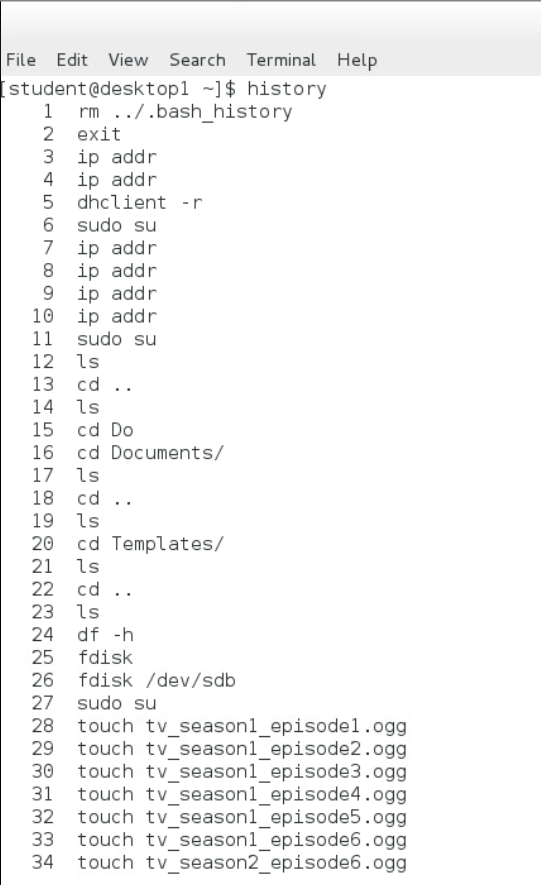
\includegraphics[scale=0.25]{Figures/2020-02-01-174110_541x885_scrot.png}
	\subcaption{CLI History pg 1}\label{Hist1}
\end{minipage}\hfill
%
\begin{minipage}[c]{0.4\linewidth}
  \centering
	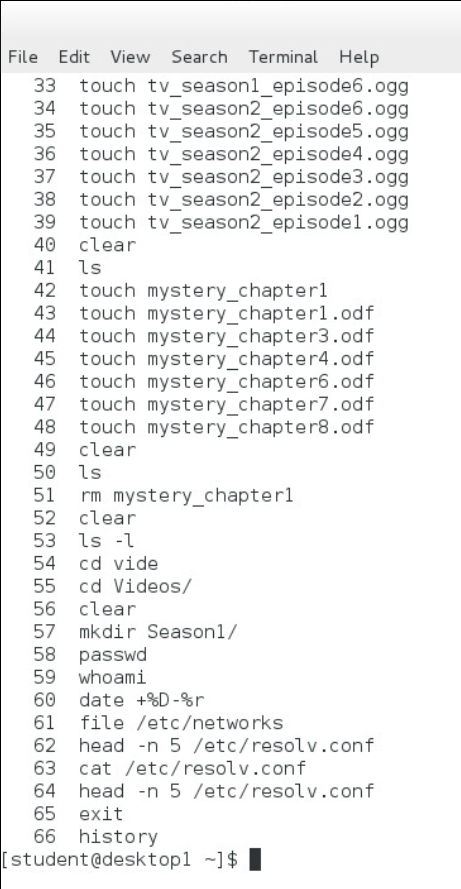
\includegraphics[scale=0.26]{Figures/2020-02-01-174125_461x889_scrot.png}
	\subcaption{CLI History pg 2}\label{Hist2}
\end{minipage}
\caption{Listing CLI History}\label{fig:Hist}
\end{figure}

\newpage

\mysection{2}{Part 2: Chapter 2 Questions}

\mysubsection{1}{List the contents of /etc/sysctl.d/ using the long listing
format. Provide the output}

\begin{center}
	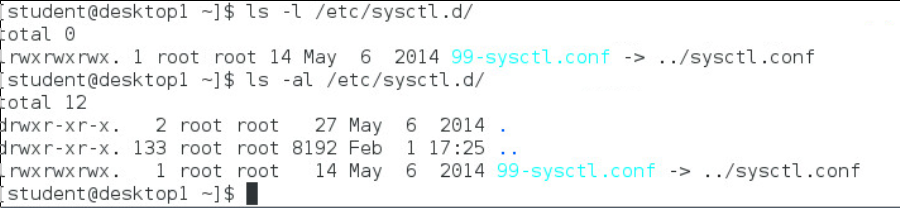
\includegraphics[scale=0.35]{Figures/2020-02-01-174628_900x208_scrot.png}
\end{center}

\mysubsection{2}{Create Two file, your firstname and your lastname, then move them to
the Documents directory. List the contents of the Documents directory. Provide the
output.}

\begin{center}
	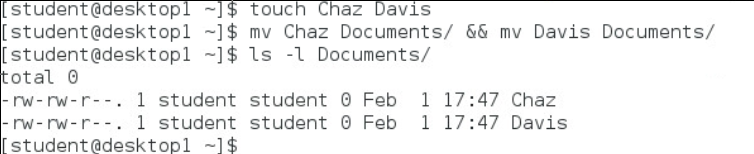
\includegraphics[scale=0.42]{Figures/2020-02-01-174852_754x154_scrot.png}
\end{center}

\mysubsection{3}{From your home directory, create a directory named CIT217 then list
the contents of your home directory. Provide the Output.}

\begin{center}
	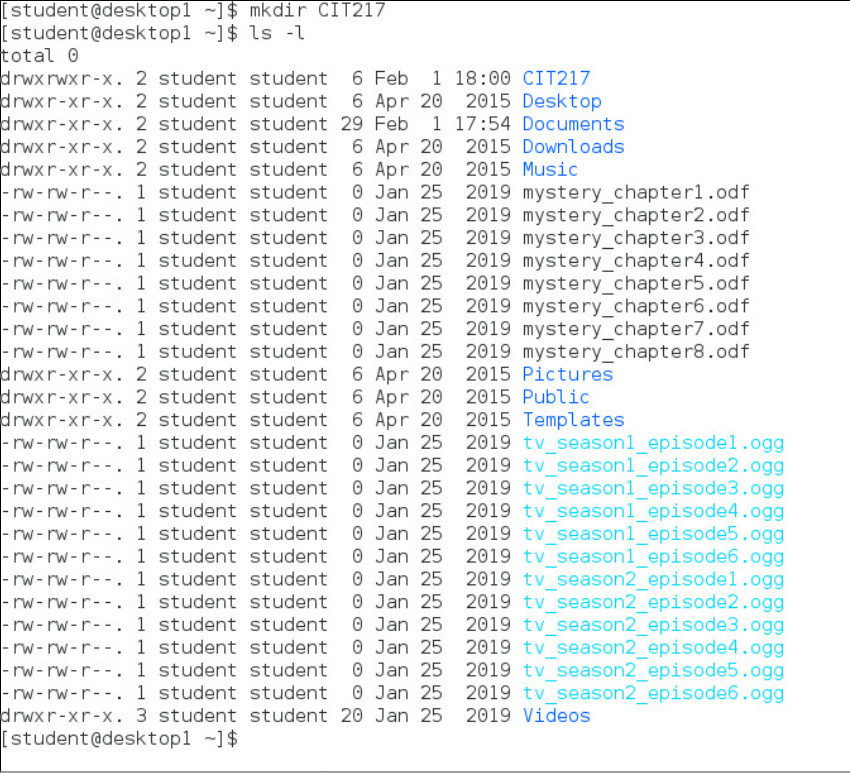
\includegraphics[scale=0.3]{Figures/2020-02-01-180028_850x773_scrot.png}
\end{center}

\mysubsection{4}{Run the command touch test{1..4}in the CLI. Using a
wildcard, copy all the test files to the Documents directory. List the contents of the
Documents directory and provide the output}
\begin{center}
	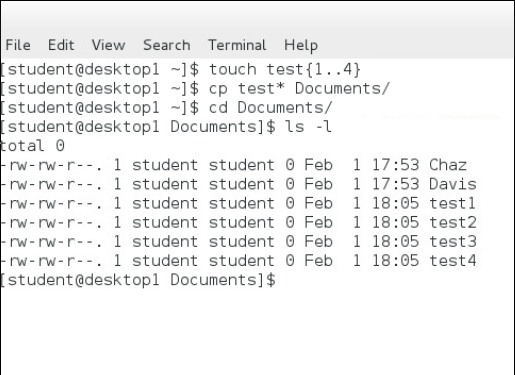
\includegraphics[scale=0.4]{Figures/2020-02-01-180610_515x375_scrot.png}
\end{center}

\end{document}

